\documentclass{article}

\usepackage[T1]{fontenc}
\usepackage{tgschola}
\usepackage{graphicx}
\usepackage{booktabs}
\usepackage{amsmath}
\usepackage{amssymb}
\usepackage{xparse}
\usepackage{stmaryrd}
\usepackage{trimclip}
\usepackage{tikz}
\usetikzlibrary{positioning,calc,arrows.meta}

\makeatletter
\DeclareRobustCommand{\shortto}{%
  \mathrel{\mathpalette\short@to\relax}%
}

\newcommand{\short@to}[2]{%
  \mkern2mu
  \clipbox{{.5\width} 0 0 0}{$\m@th#1\vphantom{+}{\shortrightarrow}$}%
  }
\makeatother

\title{Codifica delle informazioni}

\newcommand{\sym}{\text{\footnotesize simb}}
\newcommand{\msb}{\texttt{\textsc{msb}}}
\newcommand{\bin}[1]{\texttt{#1}}
\newcommand{\binn}[1]{\texttt{#1}$_2$}
\newcommand{\oct}[1]{«\texttt{#1}»$_{8}$}
\newcommand{\hex}[1]{«\texttt{#1}»$_{16}$}
\newcommand{\ds}{\!\cdot\!}
\newcommand{\fdec}[1]{{\text{{\footnotesize B10}}}\!\left(#1\right)}
\newcommand{\fn}[1]{{\text{{\footnotesize BIN}}}\!\left(#1\right)}
\newcommand{\fms}[1]{{\text{{\footnotesize MS}}}\!\left(#1\right)}
\newcommand{\fca}[1]{{\text{{\footnotesize CA1}}}\!\left(#1\right)}
\newcommand{\fcad}[1]{{\text{{\footnotesize CA2}}}\!\left(#1\right)}

\newcommand{\bitdot}{\!\cdot\!}

\ExplSyntaxOn
\NewDocumentCommand{\bits}{m}
 {
  \tl_set:Nn \l_tmpa_tl { #1 }
  \regex_replace_all:nnN { \s+ } { \c{bitdot} } \l_tmpa_tl
  \l_tmpa_tl
 }
\ExplSyntaxOff

\NewDocumentCommand{\btt}{m}
 {
  \mathtt{\bits{#1}}
 }

\NewDocumentCommand{\btta}{m}
 {
  \langle\mathtt{\bits{#1}}\rangle
 }

\begin{document}

\titlepage

\section{Alfabeti}

Quello che non mi piace degli alfabeti, è che in fondo è definito solo quello di destinazione: quello del mondo reale ne è una conseguenza. Che senso ha definirlo?
Si definiscono le regole, i simboli del mondo-computer, e si ottengono i simboli del mondo reale.


\section{Introduzione}

In generale, lo scopo della comunicazione è lo scambio di un'informazione. Questo scambio può avvenire tra qualsiasi tipo di essere: umano, animale, vegetale. Per gli essere umani, la comunicazione avviene attraverso il linguaggio, sia in forma orale che in forma scritta.%
\\[6mm]
\textbf{1)$\,$\underline{Parzialità}:} una comunicazione non \textit{trasmette} mai la realtà completa, ma solo una sua \textbf{parte}.%
\\[1mm]\noindent %
Ad esempio, quando vediamo un cane che sta correndo, possiamo trasmettere questa informazione dicendo:
\begin{quote}
    \textit{``Guarda c'è un cane che corre''}
\end{quote}
Ma questa non è una descrizione completa della realtà, infatti le seguenti domande non hanno risposta:
\begin{itemize}\setlength{\itemsep}{-0.2em}
    \item Chi è quel cane?
    \item Verso dove corre?
    \item Quanto veloce?
    \item Di che razza è?
\end{itemize}
\vspace{4mm}
\textbf{2)$\,$\underline{Interpretabilità}}: una comunicazione ricevuta da due diversi soggetti potrà essere interpretata \textbf{diversamente}.
\\[1mm]\noindent %
Rispetto l'esempio del cane, ogni ricevente potrà immaginarsi diversi scenari:
\begin{itemize}
    \item Una cane che corre in mezzo alla strada.
    \item Un cane che corre sul marciapiedi.
    \item Uno può immaginarsi un Dobermann, un altro un Chihuahua.
\end{itemize}
E tutto questo a seconda della personalità di chi riceve.
\\[6mm]
\textbf{3)$\,$\underline{Limitatezza}:} una comunicazione potrà essere effettuata utilizzando un numero finito di simboli.%
\\[1mm]\noindent %
Rispetto all'esempio di cui sopra i simboli sono le parole, e sebbene quella frase potrà essere detta in modi diversi, le parole usate saranno limitate a quelle della lingua italiana. La limitatezza nel caso degli essere umani è dovuta alla possibilità di poter conoscere solamente un numero limitato di parole.

\subsection{Esempio}

Iniziamo da un esempio. In un bar ci sono due studenti di informatica, un inglese di nome \textsc{Tom} ed un cinese di nome \textsc{Wu}, entrambi parlano solamente le proprie lingue. \textsc{Tom} vuole comunicare a \textsc{Wu} il numero \textsc{sette}. %
Per fare questo \textsc{Tom} prende un dizionario Inglese-Cinese e cerca il termine «seven» e trova che si dice «qī», e lo comunica a \textsc{Wu}:
\begin{center}
    \begin{tikzpicture}[centered]
        \node[draw, minimum width=2cm, minimum height=2.cm, align=center] (tom) at (0, 0) {\textsc{Tom}};
        \node[draw, minimum width=2cm, minimum height=2.cm, align=center] (wu) at (8cm, 0) {\textsc{Wu}};

        \node[] (dict) at ($(tom.west)!0.5!(wu.east)$) {\includegraphics[width=1cm]{dict.pdf}};

        \draw[dashed] ([yshift=0mm]tom.north) to[out=5, in=175] node[fill=white] {\textsc{sette}} ([yshift=0mm]wu.north) ;

        % \node[draw, font=\footnotesize, rounded corners] at([yshift=-5mm]tom.north) {\textsc{seven}};
        % \node[draw, font=\footnotesize, rounded corners] at([yshift=-5mm]wu.north) {\textsc{qī}};

        \draw[-{Stealth}] ([yshift=0mm]tom.east) -- ([yshift=0mm]dict.west) node[fill=white, pos=0.5] {«seven»};
        \draw[-{Stealth}] ([yshift=0mm]dict.east) -- ([yshift=0mm]wu.west) node[fill=white, pos=0.5] {«qī»};
    \end{tikzpicture}
\end{center}
%
\paragraph{Comunicare mela:} Adesso \textsc{Tom} vuole comunicare a \textsc{Wu} \textsc{mela}, e lo fa utilizzando sempre lo stesso dizionario.
\begin{center}
    \begin{tikzpicture}[centered]
        \node[draw, minimum width=2cm, minimum height=2.cm, align=center] (tom) at (0, 0) {\textsc{Tom}};
        \node[draw, minimum width=2cm, minimum height=2.cm, align=center] (wu) at (8cm, 0) {\textsc{Wu}};

        \node[] (dict) at ($(tom.west)!0.5!(wu.east)$) {\includegraphics[width=1cm]{dict.pdf}};

        \draw[dashed] ([yshift=0mm]tom.north) to[out=5, in=175] node[fill=white] {\textsc{mela}} ([yshift=0mm]wu.north) ;

        % \node[draw, font=\footnotesize, rounded corners] at([yshift=5mm]tom.south) {\textsc{apple}};
        % \node[draw, font=\footnotesize, rounded corners] at([yshift=5mm]wu.south) {\textsc{píngguǒ}};

        \draw[-{Stealth}] ([yshift=0mm]tom.east) -- ([yshift=0mm]dict.west) node[fill=white, pos=0.5] {«apple»};
        \draw[-{Stealth}] ([yshift=0mm]dict.east) -- ([yshift=0mm]wu.west) node[fill=white, pos=0.5] {«píngguǒ»};
    \end{tikzpicture}
\end{center}
Ricapitolando:
\begin{center}
    % \resizebox{5cm}{!}{%
    \begin{tabular}{@{}lccccc}
        \toprule
                & \multicolumn{2}{c}{\textsc{sette}} & \phantom{a} & \multicolumn{2}{c}{\textsc{mela}}                              \\
                & \textsc{Tom}                       & \textsc{Wu} &                                   & \textsc{Tom} & \textsc{Wu} \\\cmidrule{2-3}\cmidrule{5-6}
        Termine & «seven»                            & «qī»        &                                   & «apple»      & «píngguǒ»   \\[2mm]
        % Traduzione & \multicolumn{5}{c}{Usando un \underline{dizionario}}\\
        \bottomrule
    \end{tabular}%
    % }
\end{center}

\subsection{La lingua è un codice?}

Dato questo esempio, possiamo dire che quello che \textsc{Tom} fa è codificare il termine «seven» in «qī» ed il termine «apple» in «píngguǒ». Ma quando \textsc{Wu} ascolta «píngguǒ» gli sorge un dubbio:
\begin{quote}
    \textsc{Tom} intende il frutto?\\
    oppure \textsc{Tom} intende l'azienda Apple?
\end{quote}
Essendo sia \textsc{Tom} che \textsc{Wu} due studenti di informatica.

Questo problema può presentarsi non solo con \textsc{mela} ma con qualsiasi termine.

\paragraph{Conclusione}
Per capire il \textbf{significato} di un termine, che sia in italiano, cinese o inglese, non basta il termine stesso. Ogni termine è intrepretabile a seconda del contesto, del tono e di altri fattori.
\begin{itemize}
    \item \textsc{sette}, che può essere «seven» o «qī» è poco interpretabile (ma può sempre confondersi col film di David Fincher).
    \item \textsc{mela}, soprattutto se detto da un inglese ad un cinese, entrambi studenti di informatica, è molto interpretabile.
\end{itemize}
Nel linguaggio l'interpratibilità di ogni termine è considerato anche un vantaggio, in informatica no:
\begin{quote}
    Ogni termine in informatica deve avere un significato preciso, ovvero \underline{non interpretabile}.
\end{quote}
Quando un linguaggio è definito da termini ognuno con un preciso e non-interpretabile significato, viene detto \textbf{codice}.


\section{Codice}

In informatica il codice viene utilizzato per legare due mondi: quello reale e quello del computer. Per questo quando si parla di codice si parla anche di codifica e decodifica. La codifica è il passaggio dal mondo reale a quello del computer, la decodifica è il passaggio dal mondo del computer a quello del reale.

Nel mondo reale, come abbiamo visto precedentemente con l'esempio di \textsc{Tom} e \textsc{Wu}, un significato può assumere diverse forme. Ad esempio prendiamo il numero 10, esso può assumere diverse \textit{forme}:
\begin{itemize}\setlength\itemsep{-0.2em}
    \item «10» con i numeri arabi.
    \item «dieci» in italiano.
    \item «ten» in inglese.
    \item «X» nei numeri romani.
    \item «IIIIIIIIII» nella numerazione unaria.
    \item «1010» in base 2.
    \item «12» in base 8.
    \item «A» in base 16.
    \item «K» in base 64.
\end{itemize}
Tutte queste forme vengono dette \textbf{significanti} del significato 10.
Il numero dieci nel mondo dei computer invece diventa qualcosa definito molto precisamente:
\begin{itemize}
    \item Si stabilisce come convertirlo in binario.
    \item Si stabilisce in quanti bit.
\end{itemize}
Ora proviamo ad effettuare diverse codifiche:
\begin{itemize}\setlength\itemsep{-0.2em}
    \item 8-bit, \msb a sinistra: $\btt{0000 1010}$.
    \item 16-bit, \msb a sinistra: $\btt{0000 0000 0000 1010}$.
    \item 8-bit, \msb a destra: $\btt{0101 0000}$.
    \item 16-bit, \msb a destra: $\btt{0101 0000 0000 0000}$.
\end{itemize}
Tutte queste sono possibili codifiche del numero 10, il calcolatore dovrà poi utilizzarle sapendo a quale codifica esse appartengono.

Analizziamo ora in questi termini tutte le codifiche fin'ora viste.



Dopo aver visto varie tipologie di conversione, possiamo finalmente dare la definizione di \textit{codice}:
\begin{quote}
    Un codice è un insieme di regole per convertire una informazione in un altro oggetto o in un'altra azione, non necessariamente dello stesso tipo.
\end{quote}
Facciamo un paio di esempi:
\begin{center}
    \begin{tabular}{lp{2cm}lp{3cm}}
        \toprule
                     & \textbf{tipo di informazione} & \textbf{si trasforma in} & \textbf{come?}                                                                     \\
        \midrule
        Semaforo     & Colore                        & Azione                   & Rosso $\rightarrow$ \textit{stop};\newline verde $\rightarrow$ \textit{procedere}. \\[2mm]
        Codice Morse & Sequenza di punti/linee       & Lettera/numero           & \bin{\dots{}} $\rightarrow$ \bin{S};\newline
        \bin{{-}{-}{-}} $\rightarrow$ \bin{0};\newline
        \bin{\dots{}{-}{-}{-}\dots{}} $\rightarrow$ \bin{SOS}.                                                                                                       \\
        \bottomrule
    \end{tabular}
\end{center}
\paragraph{Conversione tra basi}
La conversione tra basi che abbiamo visto noi (tra basi 2/8/10/16) può rientrare nella definizione di codice data sopra, ma in senso molto ampio. Fintanto che convertiamo un numero tra una base ed un'altra, stiamo solamente cambiando la sua rappresentazione, e lo scopo di questa conversione, potremmo dire, non \textit{va al di là del foglio di carta in cui abbiamo effettuato la conversione}.
$\btt{1111 0000 1010 1100}$

\paragraph{Scopo}
Un codice, invece, non cambia solo la rappresentazione di una informazione, ma la cambia avendo già in mente un preciso \underline{scopo}.
Quindi:
\begin{itemize}
    \item Effettuiamo un \textbf{cambio di rappresentazione} quando convertiamo una informazione in un altra forma senza ulteriore scopo.
    \item Effettuiamo una \textbf{codifica} quando convertiamo una informazione in un'altra forma con uno scopo preciso.
\end{itemize}
Questo è coerente con gli esempi di cui sopra:
\begin{itemize}
    \item Il codice morse viene utilizzato per convertire caratteri alfanumerici in sequenze di linee e punti in quanto linee e punti, una volta convertiti in segnali radio, sono più facili e meno soggetti ad errore durante la trasmissione e la ricezione in una comunicazione radiofonica, per di più, funzionano bene anche se utilizzati in forma luminosa o sonora.
    \item Il codice \textit{semaforo} viene utilizzato per convertire un colore in una azione in quanto per un essere umano è più immediato e meno soggetto ad errore convertire un colore in un'azione\footnote{Si pensi se invece dei colori ci fossero le scritte.}.
\end{itemize}

\paragraph{Conversione in base 2} Pensiamo quindi ad una conversione del numero $125$ in base 2. Tale numero è \bin{1111101}. Questa conversione è senza scopo ulteriore, e quindi è un \textit{cambio di rappresentazione}. Se volessimo invece effettuare una codifica, dovremmo capire qual è lo \underline{scopo} di tale conversione?
Allora potremmo modificare la conversione in questo modo:
\begin{quotation}
    Convertire il numero $125$ in base 2 per un computer con un processore di 16 bit.
\end{quotation}
In questo caso il risultato diventerà: \bin{0000 0000 0111 1101}. Avendo specificato lo scopo, ovvero di essere utilizzato da un computer di 16 bit, abbiamo applicato una \textit{codifica}.
Una volta stabilito lo scopo, passare da base 2 a base 8 o base 16, non è altro che un cambio di rappresentazione, ma all'interno dello scopo definito, quindi quello di essere utilizzato con un computer con un processore di 16 bit.
Quindi, solo per quanto riguarda i numeri:
\begin{itemize}
    \item \textit{Codifica}: convertire un numero qualsiasi in qualsiasi base in un numero compatibile con l'utilizzo di un calcolatore.
    \item \textit{Cambio di rappresentazione}: convertire un numero qualsiasi in qualsiasi base in un'altra base.
\end{itemize}
Infine useremo i seguenti termini:
\begin{itemize}
    \item \textbf{Valore}: il numero come quantità astratta, cioè indipendentemente da come lo scriviamo.
    \item \textbf{Rappresentazione}: lo stesso valore può essere scritto in più modi (ad esempio base 2, base 8, base 10).
    \item \textbf{Codice}: il valore viene rappresentato in una forma compatibile ad uno specifico scopo.
\end{itemize}

\subsection{Codice numeri naturali}
I numeri naturali $\mathbb{N}$ sono i numeri interi positivi che vanno da $0$ a infinito. La codifica utilizzata converte il numero da base 10 a base 2 e aggiunge gli zeri necessari a raggiungere il numero di bit richiesti.
\paragraph{Esempio} Dato il valore $56$ rappresentato in base 10, esso potrà essere rappresentato anche come:
\begin{itemize}\setlength\itemsep{-0.2em}
    \item in base 2: «11 1000»$_2$.
    \item in base 8: «70»$_8$.
    \item in base 16: «38»$_H$.
\end{itemize}
La codifica per un computer a 16 bit sarà:
\begin{itemize}
    \item «11 1000»$_2$ a 16-bit $\rightarrow$ $\btt{\langle 0000 0000 0011 1000\rangle}$.
\end{itemize}
\paragraph{Limiti della codifica} Con questa codifica avremmo i seguenti limiti:
\begin{itemize}\setlength\itemsep{-0.2em}
    \item Numero massimo codificabile: $2^{16}-1=65535$.
\end{itemize}

\subsubsection{Rappresentazione in altre basi}
Le basi 16 e le basi 8 sono utili per \textbf{compattare} un numero binario in un formato più leggibile. Comune è l'esempio dei colori codificati in RGB a 24-bit.
In ogni caso, i computer usano sempre e solo i bit.
\textsl{Attenzione} a rappresentare diversamente $\btt{0000 0000 0011 1000}$:
\begin{itemize}\setlength\itemsep{-0.2em}
    \item In base 16 $\rightarrow$ \hex{0038}.
    \item In base 8 $\rightarrow$ \oct{00070}.
\end{itemize}
\textsc{\underline{Ma attenzione}} al procedimento inverso:
\begin{itemize}\setlength\itemsep{-0.2em}
    \item $\btt{0038}_8$ in base 2 diventa $\btt{0000 0000 0111 1101}$, che è esattamente il codice.
    \item $\btt{00070}_H$ in base 2 diventa $\btt{\underline{00} 0000 0000 0111 1101}$, che \textbf{non} è esattamente il codice in quanto abbiamo due zeri in più che \underline{non esistono} nel codice.
\end{itemize}
Per cui \underline{\textbf{si deve sempre ricordare le regole della codifica applicata.}}

\subsection{Funzioni}
Abbiamo quindi due mondi:
\begin{center}
    \resizebox{0.8\textwidth}{!}{%
        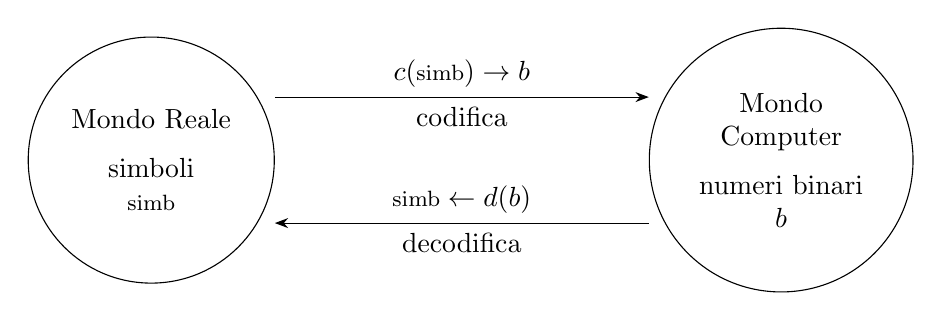
\begin{tikzpicture}
            \node[draw, circle, minimum width=2cm, text width=2.5cm, align=center] (mr) {Mondo Reale\\[2mm]simboli\\$\sym$};
            \node[draw, circle, minimum width=2cm, text width=2.5cm, align=center] (mc) at (8cm,0) {Mondo Computer\\[2mm]numeri binari\\$b$};
            \draw[-{Stealth}] ([yshift=8mm]mr.east) -- ([yshift=8mm]mc.west) node[pos=0.5,above] {$c(\sym)\rightarrow b$} node[pos=0.5,below] {codifica};
            \draw[{Stealth}-] ([yshift=-8mm]mr.east) -- ([yshift=-8mm]mc.west) node[pos=0.5,above] {$\sym \leftarrow d(b)$} node[pos=0.5,below] {decodifica};
        \end{tikzpicture}}
\end{center}
Indichiamo con:
\begin{itemize}\setlength\itemsep{-0.2em}
    \item \(c(\sym)\rightarrow b\) la funzione di codifica, che trasforma un qualsiasi simbolo $\sym$ in un numero binario $b$.
    \item $d(b) \rightarrow \sym$ la funzione di decodifica, che trasforma un qualsiasi numero binario $b$ in un simbolo $\sym$.
\end{itemize}
Nel caso della codifica con numeri interi precedente avremmo:
\begin{itemize}\setlength\itemsep{-0.2em}
    \item $\sym$: numeri interi.
    \item $b$: numeri binari a $n$-bit.
    \item $c(\sym)$: conversione da base 10 a base 2.
\end{itemize}


\subsubsection{Funzione da base10 a base2}
Definiamo la seguente funzione
\begin{equation*}
    f^n_{10\shortto{} 2}(d)
\end{equation*}
la funzione che riceve in input un numero decimale e lo converte in un numero binario a $n$ bit.
Esempio:
\begin{align*}
    f(13)      & = \bits{1101}                \\
    f^{5}(13)  & = \bits{0 1101}              \\
    f^{16}(13) & = \bits{0000 0000 0000 1101}
\end{align*}
Se $n$ non è definito, allora si userà il minor numero possibile di bit necessari.




\section{Numeri interi con segno}
Con la codifica dei numeri naturali è impossibile codificare il simbolo $-$, dato che nel mondo dei computer esistono solamente i numeri binari. Per cui è necessario utilizzare un diverso tipo di codifica. Per codificare i numeri relativi (ovvero sia maggiori che minori di zero) le seguenti sono le codifiche principali:
\begin{itemize}\setlength\itemsep{-0.2em}
    \item Modulo e segno.
    \item Complemento a 1.
    \item Complemento a 2.
\end{itemize}

\paragraph{Numeri positivi} Per quanto riguarda i numeri \underline{positivi}, tutte e tre le codifiche --una volta stabilito il numero di bit-- usano la stessa funzione $c(\sym)$, quella dei numeri naturali. Per cui il valore $+56$ codificato per un calcolatore di 16 bit sarà
\begin{equation*}
    +56 \rightarrow \btt{0000 0000 0111 1101}_{2}
\end{equation*}
per tutte e tre le codifiche.



%%%%%%%%%%%%%%%%%%%%%%%%%%%%%%%%%%%%%%%%%%%%%%%%%%%%%%%%%%%%%%%%%%%%%%%%%%%%
\subsection{Modulo e segno}
Nella codifica ``Modulo e segno'' il \msb{} viene utilizzato per indicare il segno:
\begin{itemize}
    \item \msb{} $=0$: allora avremo segno $+$ (numero positivo).
    \item \msb{} $=1$: allora avremo segno $-$ (numero negativo).
\end{itemize}
Definiamo la funzione
\begin{equation*}
    \fms{b}
\end{equation*}
la quale richiede come input un numero binario $b$ e ne inverte il \texttt{MSB} (ovvero la prima cifra da sinistra).
Esempi:
\begin{align*}
    \fms{\btt{\underline{0}010}}       & = \btt{\underline{1}010}       \\
    \fms{\btt{\underline{1}011000010}} & = \btt{\underline{0}011000010}
\end{align*}

\paragraph{Regole codifica}
\begin{itemize}\setlength\itemsep{-0.2em}
    \item Nel caso dei numeri positivi, si convertono utilizzando $\fn{\sym}$.
    \item Nel caso dei numeri negativi, si convertono utilizzando $\fms{\fn{\sym}}$.
\end{itemize}
\textsc{Esempio numero negativo:} Dato il numero $-56$, lo si vuole codificare per l'utilizzo con un calcolatore a 16 bit:
\begin{itemize}\setlength\itemsep{-0.2em}
    \item Si converte il numero senza segno $56$ in binario a 16 bit:
          \[
              b = \fn{56} \rightarrow \btta{0000 0000 0011 1000}
          \]
    \item  Si applica la funzione $\fms{}$:
          \begin{align*}
              \fms{b} = \btt{\underline{1}000 0000 0011 1000}
          \end{align*}
\end{itemize}

\paragraph{Decodifica} Per decodificare, ovvero passare da codice binario a simbolo, si devono effettuare due passaggi:
\begin{enumerate}\setlength\itemsep{-0.2em}
    \item Capire se il numero è negativo: \msb{} uguale a 1.
    \item Calcolare il modulo applicando $\fdec{\fms{b}}$.
\end{enumerate}
Esempio:
\begin{itemize}\setlength\itemsep{-0.2em}
    \item Numero positivo $b=\btta{0000 0011 1110 1000}$:
          \[
              \sym = \fdec{b} \rightarrow 1000
          \]
    \item Numero negativo $b=\btta{1000 0011 1110 1000}$:
          \begin{align*}
              \sym = \fdec{\fms{b}} \rightarrow              \\
              \rightarrow & \fdec{\btt{0111 1100 0001 0111}} \\
              \rightarrow & -1000
          \end{align*}
\end{itemize}

\paragraph{Limiti}
\begin{itemize}\setlength\itemsep{-0.2em}
    \item Dato che il \msb{} è utilizzato per indicare il segno, solamente 15 bit dei 16 bit possono essere utilizzati per il valore numerico, quindi il \underline{massimo} numero codificabile sarà: $2^{15}-1=32767$.
    \item E lo stesso vale per il numero più piccolo: $-2^{15}+1=-32767$.
    \item Si ha una doppia rappresentazione dello zero:
          \begin{align*}
              +0 \rightarrow \btt{0000 0000 0000 0000} \\
              -0 \rightarrow \btt{1000 0000 0000 0000}
          \end{align*}
\end{itemize}

%%%%%%%%%%%%%%%%%%%%%%%%%%%%%%%%%%%%%%%%%%%%%%%%%%%%%%%%%

%%%%%%%%%%%%%%%%%%%%%%%%%%%%%%%%%%%%%%%%%%%%%%%%%%%%%%%%%
\subsection{Complemento a 1}
Con la codifica ``Complemento a 1'' si codificano i numeri negativi invertendo\footnote{Con \textit{invertire} si intende che gli \texttt{0} diventano \texttt{1} e gli \texttt{1} diventano \texttt{0}.} tutti i bit del numero positivo. Esempio a 16 bit:
\begin{align*}
    +10 \rightarrow \btt{0000 0000 0000 1010} \\
    -10 \rightarrow \btt{1111 1111 1111 0101}
\end{align*}
Definiamo la funzione
\begin{equation*}
    \fca{b}
\end{equation*}
la quale richiede come input un numero binario $b$ e ne inverte tutti i bit.

\paragraph{Codifica ``Complemento a 1''}
Dato il numero $-56$, lo si vuole codificare per l'utilizzo con un calcolatore a 16 bit:
\begin{itemize}\setlength\itemsep{-0.2em}
    \item Si converte il numero senza segno $56$ in binario a 16 bit:
          \[
              56 \rightarrow \btta{0000 0000 0011 1000}.
          \]
    \item  Si applica la funzione $\fca{}$:
          \begin{align*}
              \fca{\btt{0000 0000 0011 1000}} = \btta{1111 1111 1100 0111}.
          \end{align*}
\end{itemize}
%
\paragraph{Regole}
\begin{itemize}\setlength\itemsep{-0.2em}
    \item Nel caso dei numeri positivi, si convertono utilizzando $\fn{\sym}$.
    \item Nel caso dei numeri negativi, si convertono utilizzando $\fca{\fn{\sym}}$.
\end{itemize}
\paragraph{Limiti}
\begin{itemize}\setlength\itemsep{-0.2em}
    \item Possiamo applicare la funzione $\fca{}$ solamente a metà dei numeri (quelli che con \msb{}$=0$), per cui il \underline{massimo} numero codificabile sarà: $2^{15}-1=32767$.
    \item Lo stesso vale per il numero più piccolo: $-2^{15}+1=-32767$.
    \item Si ha una doppia rappresentazione dello zero:
          \begin{align*}
              +0 \rightarrow \btt{0000 0000 0000 0000} \\
              -0 \rightarrow \btt{1111 1111 1111 1111}
          \end{align*}
\end{itemize}
\paragraph{Perché solo ai numeri con \textsc{MSB}=1?}
Se applicassimo $\fca{}$ anche ai numeri con \msb$=1$ riotterremmo codici che rappresentano i numeri positivi. Ad esempio il numero $40000$:
\[
    \fn{40000} \rightarrow \btt{1001 1100 0100 0000}
\]
Ora applichiamo $\fca{}$:
\[
    \fca{\btt{1001 1100 0100 0000}} \rightarrow \btt{0110 0011 1011 1111}
\]
che però \underline{rappresenta già} $25535$.

\paragraph{Decodifica} Per decodificare, ovvero passare da codice binario a simbolo, si devono effettuare due passaggi:
\begin{itemize}\setlength\itemsep{-0.2em}
    \item Capire se il numero è negativo: \msb{} uguale a 1.
    \item Calcolare il modulo applicando $\fdec{\fca{b}}$.
\end{itemize}
Esempio:
\begin{itemize}\setlength\itemsep{-0.2em}
    \item Numero positivo, $\btta{0000 0011 1110 1000}$:
          \[
              \fdec{\btt{0000 0011 1110 1000}} \rightarrow 1000
          \]
    \item Numero negativo, $\btta{1000 0011 1110 1000}$:
          \begin{align*}
                          & \fdec{\fca{\btt{1000 0011 1110 1000}}} \rightarrow \\
              \rightarrow & \fdec{\btt{0111 1100 0001 0111}}                   \\
              \rightarrow & -31767
          \end{align*}
\end{itemize}
%%%%%%%%%%%%%%%%%%%%%%%%%%%%%%%%%%%%%%%%%%%%%%%%%%%%%%%%%

%%%%%%%%%%%%%%%%%%%%%%%%%%%%%%%%%%%%%%%%%%%%%%%%%%%%%%%%%
\subsection{Complemento a 2}
Con la codifica ``Complemento a 2'' si codificano i numeri negativi applicando la codifica ``Complemento a 1'' e poi sommando $\btt{1}$. Esempio a 16 bit:
\begin{align*}
    +10 \rightarrow & \btt{0000 0000 0000 1010}   \\
    -10 \rightarrow & \btt{1111 1111 1111 0101} + \\
                    & \btt{0000 0000 0000 0001}=  \\
                    & \btt{1111 1111 1111 0110}   \\
\end{align*}
Definiamo la funzione
\begin{equation*}
    \fcad{b}=\fca{b} + \btt{1}
\end{equation*}
la quale richiede come input un numero binario $b$ e ne inverte tutti i bit.

\paragraph{Esempio}
Codifica ``Complemento a 1'' di $-56$ per l'utilizzo con un calcolatore a 16 bit:
\begin{itemize}\setlength\itemsep{-0.2em}
    \item Si converte il numero senza segno $56$ in binario a 16 bit:
          \[
              56 \rightarrow \btta{0000 0000 0011 1000}.
          \]
    \item  Si applica la funzione $\fca{}$:
          \begin{align*}
              \fca{\btt{0000 0000 0011 1000}} = \btta{1111 1111 1100 0111}.
          \end{align*}
    \item  Si somma $\btt{1}$:
          \begin{align*}
              \btta{1111 1111 1100 0111} + 1 = \btta{1111 1111 1100 1000}.
          \end{align*}
\end{itemize}
%
\paragraph{Regole}
\begin{itemize}\setlength\itemsep{-0.2em}
    \item Nel caso dei numeri positivi, si convertono utilizzando $\fn{\sym}$.
    \item Nel caso dei numeri negativi, si convertono utilizzando $\fcad{\fn{\sym}}$.
\end{itemize}
\paragraph{Limiti}
\begin{itemize}\setlength\itemsep{-0.2em}
    \item Possiamo applicare la funzione $\fca{}$ solamente ai numeri con \msb{}$=0$, per cui il \underline{massimo} numero codificabile sarà: $2^{15}-1=32767$.
    \item Non vale lo stesso per il numero più piccolo grazie alla somma i $\btt{1}$, infatti sarà: $-2^{15}+1=-32768$.
    \item Non si ha una doppia rappresentazione dello zero.
\end{itemize}

\paragraph{Perché non si ha una doppia rappresentazione dello zero?}
Applichiamo il procedimento inverso a $\btt{1111 1111 1111 1111}$:
\begin{itemize}
    \item Sommiamo uno ottenendo $\btta{0000 0000 0000 0000}$.
    \item $\fca{\btt{0000 0000 0000 0000}} \rightarrow \btt{1111 1111 1111 1111}$.
\end{itemize}
Per cui otteniamo che $\btt{1111 1111 1111 1111} \rightarrow -32768$.

\subsection{Numeri interi (complemento a 2)}
Definiamo la funzione
\begin{equation*}
    f_{\text{\tiny{CA2}}}(n) = f_{\text{\tiny{CA1}}}(n) + \mathtt{1}
\end{equation*}
Esempi:
\begin{align*}
    f_{\text{\tiny{CA2}}}(\mathtt{0010})       & = \mathtt{1101} + \mathtt{1} = \mathtt{1110} \\
    f_{\text{\tiny{CA1}}}(\mathtt{0011000010}) & = \mathtt{1100111101} + \mathtt{1}           \\
                                               & = \mathtt{1100111110}
\end{align*}
La codifica complemento a 2 è la seguente:
\begin{itemize}
    \item Se il numero è maggiore di zero si converte da base10 a base2.
    \item Se il numero è minore di zero si utilizza $f_{\text{\tiny{CA2}}}(n)$.
\end{itemize}
% Dati i numeri \(125\) e $-125$.\\
Codifica di $-125$ per l'utilizzo con un calcolatore a 16 bit (complemento a 2):
\begin{align*}
     & f_{\text{\tiny CA1}}(\mathtt{0000000001111101})_{2}+\mathtt{1}= \\
     & =\mathtt{1111111110000010}_{2} + 1=                             \\
     & =\mathtt{1111111110000011}_{2}
\end{align*}
Cambio di rappresentazione del codice di cui sopra:
\begin{itemize}
    \item da base 2 a base 16: \(0000000001111101_{2}=007D_{16}\);
          \quad \(1111111110000011_{2}=FF83_{16}\).
    \item da base 2 a base 8: \(0000000001111101_{2}=000175_{8}\);
          \quad \(1111111110000011_{2}=177603_{8}\).
\end{itemize}

\emph{attenzione:} quando si cambia la rappresentazione del codice, non
bisogna mai dimenticare lo \emph{scopo} (rappresentare su 16 bit in
complemento a 2):

\begin{itemize}
    \item
          lo riporto in binario (mantenendo 16 bit): ritorna esattamente lo
          stesso.
    \item
          lo riporto in binario dall'ottale: ottengo 18 bit (6 cifre ottali),
          quindi devo scartare i 2 bit in più a sinistra e mantenere solo i 16
          bit meno significativi.
\end{itemize}


\section{Codifica binaria dei numeri}

\subsection{Numeri interi}

Calcoliamo il numero $125$ in base 10 in un numero in base 2. Il procedimento è quello di eseguire la divisione per 2 e raccogliere i resti:
\begin{center}
    \begin{tabular}{r|ll@{ }l}
        125 & 2 & = 62 & + \textbf{1} \\
        62  & 2 & = 31 & + \textbf{0} \\
        31  & 2 & = 15 & + \textbf{1} \\
        15  & 2 & =  7 & + \textbf{1} \\
        7   & 2 & =  3 & + \textbf{1} \\
        3   & 2 & =  1 & + \textbf{1} \\
        1   & 2 & =  0 & + \textbf{1} \\
    \end{tabular}
\end{center}
Quindi il numero $125$ in base 2 sarà: \bin{1111101}, raccogliendo i resti dall'ultima riga fino alla prima.



Informatica:
\begin{itemize}
    \item Elaborazione (in loco): come l'informazione esiste e viene gestita dentro un sistema.
          \begin{itemize}
              \item Memorizzazione (RAM, file system, database, caching).
              \item Trasformazione/decisione (algoritmi, computazione, OS, compilatori, ML).
              \item Affidabilità locale (concorrenza, consistenza, isolamenti, crash recovery).
              \item Rappresentazione (bit, tipi, formati, strutture dati).
          \end{itemize}
    \item Comunicazione: come l'informazione passa tra sistemi/processi.
          \begin{itemize}
              \item Protocolli, reti, distribuzione, sincronizzazione, web.
              \item Sicurezza “in transito” (TLS, autenticazione, integrità, ecc.).
          \end{itemize}
\end{itemize}


Comunicazione richiede la codifica, la quale può essere:
\begin{itemize}
    \item A lunghezza fissa.
    \item A lunghezza variabile.
\end{itemize}

\begin{itemize}
    \item Significante: 10, 1010, 0x0A, 12.
    \item Codifica: Numeri arabi in base 10, base2, base16, base8.
    \item Significato: dieci, dieci, dieci, dieci.
\end{itemize}

\begin{itemize}
    \item Insieme dei dati da rappresentare:
          \begin{itemize}
              \item Alfabeto sorgente ($T$).
              \item Composto da $n$ elementi (cardinalità $n=\left|T\right|$).
              \item \textit{Esempio}: numeri fino a mille, tutti i numeri reali.
          \end{itemize}
    \item Insieme dei simboli:
          \begin{itemize}
              \item Alfabeto codice ($E$).
              \item Composto da $k$ elementi (cardinalità $k=\left|E\right|$).
              \item \textit{Esempio}: lettere dell'alafabeto, 0/1 dei numeri binari.
          \end{itemize}
    \item Una sequenza di simboli dell'alfabeto $E$ è detta \textbf{stringa}.
    \item Passare da un dato/significato ad un significante, ovvero una sequenza di simboli, è detto codifica o trasformazione (funzioni di).
\end{itemize}

Codici ridondanti:
\begin{itemize}
    \item
\end{itemize}
\end{document}